\documentclass[11pt]{article}
\usepackage[margin=1in]{geometry}
\usepackage[T1]{fontenc}
\usepackage[utf8]{inputenc}
\usepackage{lmodern}
\usepackage{graphicx}
\usepackage{booktabs}
\usepackage{longtable}
\usepackage{array}
\usepackage{amsmath, amssymb}
\usepackage{hyperref}
\usepackage{xcolor}
\usepackage{enumitem}
\usepackage{caption}
\usepackage{subcaption}
\usepackage{float}
\usepackage{setspace}
\usepackage{fancyhdr}

\hypersetup{
  colorlinks=true,
  linkcolor=blue!50!black,
  urlcolor=blue!50!black,
  pdftitle={Technical White Paper: OxyFormer},
  pdfauthor={Brandon Chew, Isha Jain, Hani Goodarzi}
}

\input{generated/macros.tex}

\setlength{\parskip}{0.5em}
\setlength{\parindent}{0pt}
\onehalfspacing
\pagestyle{fancy}
\fancyhf{}
\fancyhead[L]{Technical White Paper}
\fancyhead[R]{Arc Institute}
\fancyfoot[C]{\thepage}
\setlength{\headheight}{14pt}

\title{Technical White Paper:\\OxyFormer: Causal AI for Altitude-Derived Hypoxia Burden and Cancer Outcomes}
\author{Brandon Chew \and Isha Jain \and Hani Goodarzi}
\date{March 6, 2026}

\begin{document}
\pagenumbering{roman}

\begin{titlepage}
\centering
\vspace*{1.2cm}
{
\includegraphics[width=0.34\textwidth]{Arc-logo-slate.jpg}\\[1.3cm]}
{\Large OxyFormer Technical White Paper\\[0.6cm]}
{\huge \bfseries OxyFormer: Causal AI for Altitude-Derived Hypoxia Burden and Cancer Outcomes\\[0.7cm]}
{\Large Brandon Chew \quad Isha Jain \quad Hani Goodarzi\\[0.4cm]}
{\large Arc Institute\\[0.8cm]}
\vfill
\begin{minipage}{0.9\textwidth}
\centering
\textbf{Program thesis.} We built OxyFormer, a modern causal-AI prototype that combines physiologic treatment engineering, attention-based tabular transformer pretraining, transferred county embeddings, and orthogonalized continuous-treatment effect estimation. The purpose of this document is twofold: first, to describe the implemented system rigorously; second, to show why the current county-level prototype de-risks a larger person-level study with direct oxygen and health measurements from wearable or digital-health partners.
\end{minipage}
\vfill
{\large March 6, 2026}
\end{titlepage}

\pdfbookmark[1]{Abstract}{abstract}
\begin{abstract}
We study whether altitude-derived hypoxia burden is associated with lower county-level cancer incidence and mortality after adjustment for high-dimensional socioeconomic, behavioral, and public-health covariates. The technical contribution is not a single regression model. Instead, the repository now implements a multi-stage causal-AI pipeline: (i) physiologic treatment engineering from elevation to inspired oxygen proxy and normalized hypoxia burden; (ii) county feature fusion across local covariates, ACS, PLACES, SVI, and RUCC sources; (iii) self-supervised pretraining of a real attention-based tabular transformer with dual masked views, auxiliary public-health heads, and embedding-consistency regularization; and (iv) transfer of the learned county embedding into a partial-linear double-machine-learning (DML) causal head with cross-fitted orthogonal nuisance estimation.

The current transformer is trained on \CountyRows{} counties with \FoundationInputDim{} input channels, a token width of \FoundationTokenDim{}, \FoundationLayers{} self-attention layers, \FoundationHeads{} attention heads, and a \FoundationEmbeddingDim{}-dimensional county embedding. When these embeddings are appended to the curated feature set and passed into the DML stage, the estimated effect of moving hypoxia burden from the 10th to the 90th percentile is \IncidenceTotalPct{} of the mean all-cancer incidence rate and \MortalityTotalPct{} of the mean all-cancer mortality rate. Site-level analyses reveal substantial heterogeneity, with strong negative incidence effects in lung and bronchus, colon and rectum, and breast cancer, but mixed mortality behavior across sites.

This paper argues that the county prototype is already technically fundable. It defines an explicit intervention-style treatment, demonstrates an aggressive modern representation model, and provides a direct path to a larger longitudinal study with direct oxygen saturation, sleep, activity, geography, and oncology outcomes.
\end{abstract}

\tableofcontents
\newpage
\pagenumbering{arabic}

\section{Introduction and program thesis}
The motivating question is causal rather than merely predictive: what happens to cancer burden when oxygen exposure is shifted along a physiologically meaningful axis? In this repository, that axis is encoded as a county-level continuous treatment derived from altitude and inspired oxygen pressure. The broader program hypothesis is that chronic oxygen availability may act as a biologically relevant environmental exposure, but the current study is designed as an engineering prototype for causal AI rather than as a definitive epidemiologic answer.

The paper emphasizes four design principles. First, the treatment must be engineered from first principles rather than treated as a raw geographic covariate. Second, modern AI should enter the system as a reusable representation learner for heterogeneous tabular data. Third, the causal estimand must remain explicit, which means the learned representation is transferred into an orthogonalized DML stage instead of replacing the estimand with black-box prediction. Fourth, the output should be actionable for fundraising: the current county system should make it obvious why direct oxygen and longitudinal health measurements are the right next data modality.

\subsection{Implemented technical contributions}
\begin{itemize}[leftmargin=1.4em]
  \item A physiologic treatment engineering layer that converts county elevation into inspired oxygen proxy and normalized hypoxia burden.
  \item A multi-source county feature matrix spanning \ModelFeatures{} curated model features and \ModelMatrixFeatures{} model-matrix columns after preprocessing.
  \item A real tabular transformer pretrained with masked-view self-supervision and auxiliary health prediction, yielding a \FoundationEmbeddingDim{}-dimensional county embedding.
  \item A partial-linear DML estimator that uses the transferred embedding in the nuisance models for both treatment and outcome regression.
  \item Site-level heterogeneity analysis across supported incidence and mortality endpoints.
\end{itemize}

\section{Problem formulation and estimands}
For county $i$, let $T_i$ denote hypoxia burden, $Y_i$ denote a cancer endpoint, $M_i$ denote mediator candidates such as diabetes and obesity burden, and $X_i$ denote the remaining confounder vector. The primary estimand is a continuous-treatment partial effect under a partially linear structural model,
\begin{align}
Y_i &= \theta T_i + g(X_i^*) + \varepsilon_i, \\
T_i &= m(X_i^*) + \nu_i,
\end{align}
where $X_i^* = [X_i, z_i]$ augments the curated covariates with the learned county embedding $z_i$.

The total-effect models exclude mediator proxies from $X_i^*$, while the direct-effect models include them, so the estimands differ by adjustment set. This is not a full mediation analysis, but it is a useful sensitivity analysis that separates a broad total association from a more controlled direct-effect contrast.

Cross-fitted orthogonalization follows the standard residual-on-residual construction. Let $\hat g^{-k(i)}(\cdot)$ and $\hat m^{-k(i)}(\cdot)$ denote nuisance fits trained without fold $k(i)$. Then
\begin{align}
\tilde Y_i &= Y_i - \hat g^{-k(i)}(X_i^*), \\
\tilde T_i &= T_i - \hat m^{-k(i)}(X_i^*), \\
\hat\theta &= \frac{\sum_i \tilde T_i \tilde Y_i}{\sum_i \tilde T_i^2}.
\end{align}
This orthogonal score keeps the causal target explicit while still allowing flexible machine learning inside the nuisance regressions.

\section{Treatment engineering and county data fusion}
The treatment is derived from elevation $h_i$ using the standard-atmosphere approximation implemented in the repository:
\begin{align}
P_i &= P_0 \left(1 - 2.25577 \times 10^{-5} h_i\right)^{5.25588}, \\
\mathrm{PIO}_2(i) &= F_{\mathrm{IO}_2} \left( 7.50061683 \cdot P_i - 47.0 \right), \\
T_i &= 1 - \frac{\mathrm{PIO}_2(i)}{\mathrm{PIO}_2(0)}.
\end{align}
Here $P_i$ is pressure in kPa, $\mathrm{PIO}_2(i)$ is inspired oxygen proxy in mmHg, and $T_i$ is normalized hypoxia burden relative to sea level.

The county covariate system then merges local baseline features with public covariates from ACS, PLACES, SVI, and RUCC. Missingness indicators are retained as explicit channels rather than silently dropping sparse records. This is critical for the transformer stage because the masked-view pretraining objective can leverage structured missingness patterns rather than treating them as preprocessing noise.

\begin{figure}[H]
  \centering
  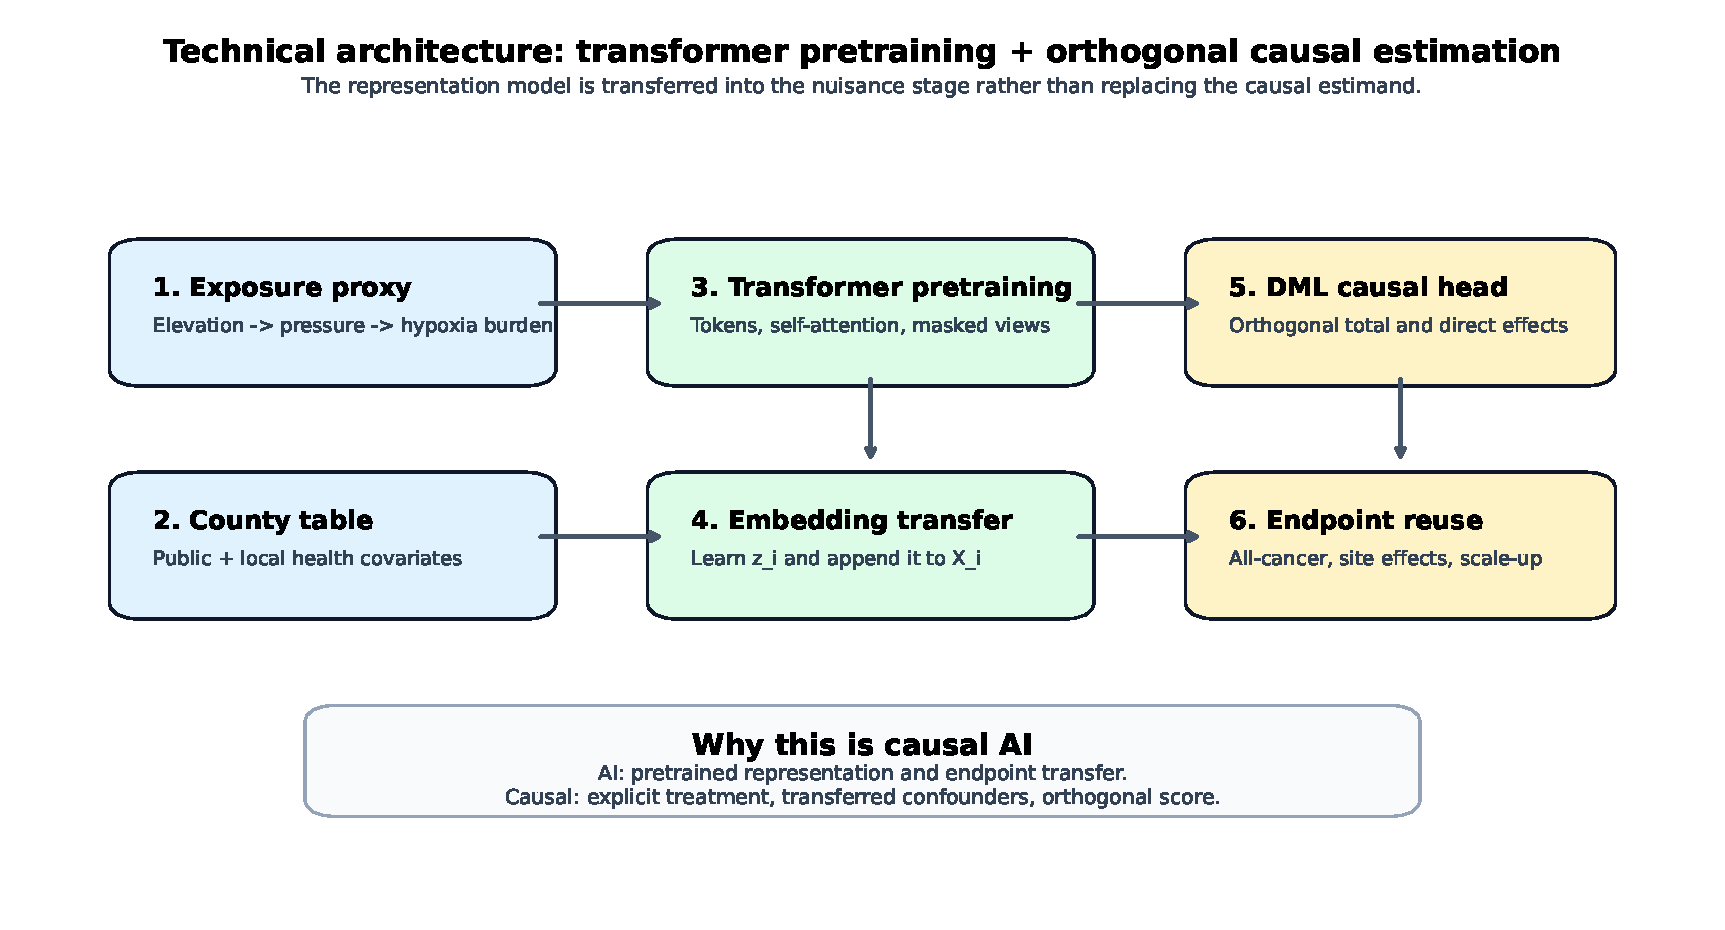
\includegraphics[width=0.96\textwidth]{../outputs/report/paper_assets/technical_architecture.pdf}
  \caption{Implemented causal-AI architecture. The attention-based tabular encoder is pretrained first; the resulting county embedding is then transferred into the orthogonal DML causal head.}
\end{figure}

\section{Attention-based tabular transformer pretraining}
The representation model is intentionally modern and intentionally aggressive. The goal is to learn a reusable county state representation before fitting the causal estimand. For each scalar feature $x_{ij}$, the model learns a token embedding through a feature-specific linear map,
\begin{align}
 e_{ij} = x_{ij} w_j + b_j,
\end{align}
then prepends a learned classification token to form the sequence
\begin{align}
S_i^{(0)} = [\mathrm{CLS}, e_{i1}, e_{i2}, \ldots, e_{ip}].
\end{align}
A stack of self-attention blocks processes the sequence,
\begin{align}
S_i^{(\ell+1)} = \mathrm{TransformerBlock}_{\ell}(S_i^{(\ell)}), \qquad z_i = \mathrm{MLP}(h^{(L)}_{i,\mathrm{CLS}}),
\end{align}
where $z_i \in \mathbb{R}^{\FoundationEmbeddingDim{}}$ is the learned county embedding.

The pretraining objective uses two independently masked views of the same county table row. Let $X_i^{(a)}$ and $X_i^{(b)}$ denote the two masked views. The shared encoder is trained with a reconstruction term, an auxiliary supervised term on public-health targets, an embedding penalty, and a consistency term:
\begin{align}
\mathcal{L} &= \mathcal{L}_{\mathrm{mask}}(\hat X_i^{(a)}, X_i) + \mathcal{L}_{\mathrm{mask}}(\hat X_i^{(b)}, X_i) \\
&\quad + \lambda_{\mathrm{aux}} \mathcal{L}_{\mathrm{aux}}(\hat y_i^{\mathrm{aux}}, y_i^{\mathrm{aux}})
+ \lambda_{\mathrm{con}} \lVert q(z_i^{(a)}) - q(z_i^{(b)}) \rVert_2^2
+ \lambda_{\mathrm{emb}} \lVert z_i \rVert_2^2.
\end{align}
This design is closer to contemporary self-supervised representation learning than to classical factor analysis or PCA. The consistency term is especially useful here because the same county should map to a stable representation under multiple masked views of the same tabular record.

\begin{table}[H]
\centering
\caption{Implemented transformer configuration}
\resizebox{\textwidth}{!}{%
\begin{tabular}{rrrrrrrrrr}
\toprule
Rows & Inputs & Embed & Token & Layers & Heads & Epochs & Mask rate & Aux targets & Final loss \\
\midrule
\CountyRows{} & \FoundationInputDim{} & \FoundationEmbeddingDim{} & \FoundationTokenDim{} & \FoundationLayers{} & \FoundationHeads{} & \FoundationEpochs{} & \FoundationMaskRate{} & \FoundationAuxTargets{} & \FoundationLoss{} \\
\bottomrule
\end{tabular}%
}
\end{table}

The current run trains for \FoundationEpochs{} epochs with a mask rate of \FoundationMaskRate{}, supervises \FoundationAuxTargets{} auxiliary health targets, and reaches a final total loss of \FoundationLoss{}. The training-curve figure shows that the representation model converges smoothly rather than simply memorizing a single objective channel.

\begin{figure}[H]
  \centering
  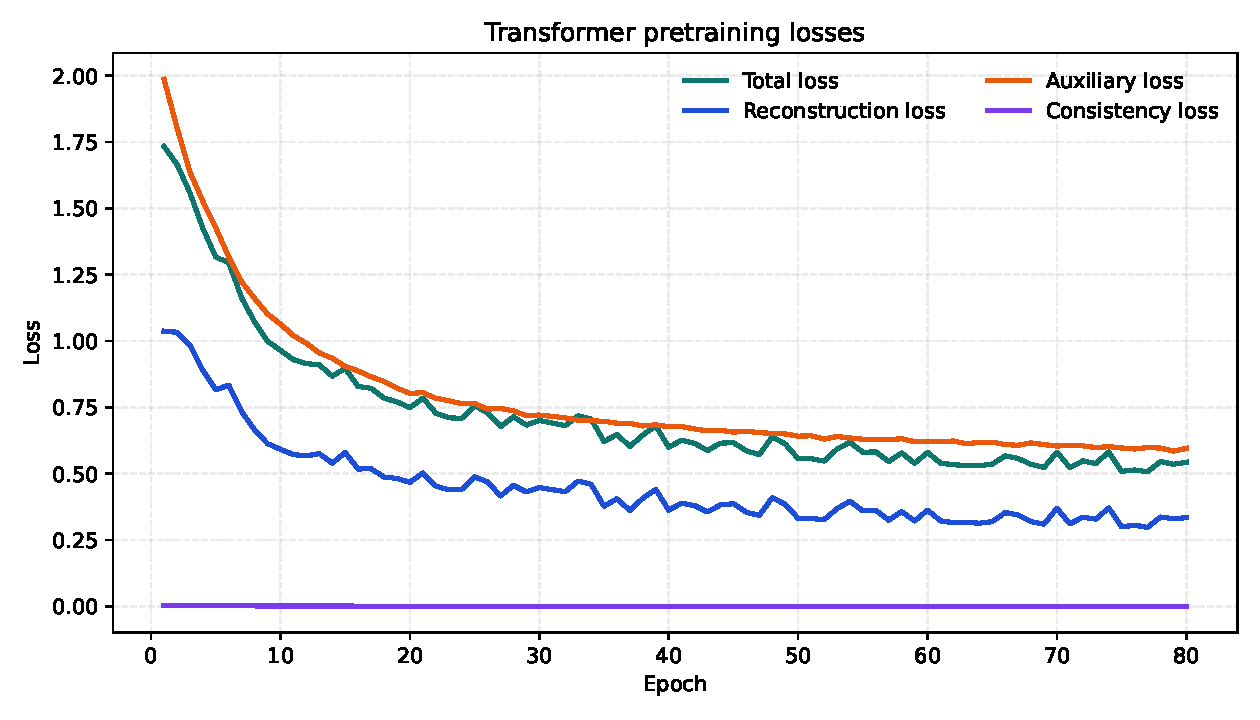
\includegraphics[width=0.82\textwidth]{../outputs/report/paper_assets/foundation_training_losses.pdf}
  \caption{Pretraining losses for the dual-view masked tabular transformer. Total, reconstruction, auxiliary, and consistency losses all decline over training.}
\end{figure}

\section{Transferred embeddings in the causal head}
The central causal-AI design choice is to transfer the learned representation into the nuisance stage, not to replace the estimand with a black-box prediction objective. After pretraining, each county receives a fixed embedding $z_i$, and the nuisance feature set becomes
\begin{align}
X_i^* = [X_i, z_i].
\end{align}
The outcome and treatment regressions are then fit with ridge-regularized learners inside cross-fitting. This is a conservative choice for the causal head. The representation learner is expressive; the final orthogonal stage is intentionally more stable.

This separation matters scientifically. If the transformer were directly fine-tuned to maximize predictive performance on the cancer endpoints, the analysis would collapse into a pure prediction exercise. By placing the transformer inside the nuisance pipeline, the learned representation contributes to confounder adjustment and variance reduction while preserving a transparent intervention-style estimand.

\section{Experimental configuration}
The full system operates on \CountyRows{} counties for representation pretraining, with primary all-cancer models estimated on \IncidenceN{} counties for incidence and \MortalityN{} counties for mortality. The Phase 3 causal head uses 5-fold cross-fitting with ridge penalties $\alpha_Y = 25$ and $\alpha_T = 10$. State fixed effects are encoded as dummy variables where coverage allows.

This configuration is not meant to be the last word in model selection. It is meant to prove that the repository can already support a genuinely modern stack: aggressive self-supervised representation learning on structured public-health data, coupled to a formally defined orthogonal causal estimator.

\section{Primary results}
The all-cancer analysis shows a persistent negative association between higher hypoxia burden and both incidence and mortality after adjustment. The magnitude is easiest to interpret through the 10th-to-90th percentile treatment shift. For the all-cancer models, that contrast corresponds to \IncidenceTotalPct{} of the mean incidence rate for the total-effect estimand and \IncidenceDirectPct{} for the direct-effect estimand. For mortality, the corresponding values are \MortalityTotalPct{} and \MortalityDirectPct{}.

\begin{table}[H]
\centering
\caption{Primary all-cancer causal estimates}
\resizebox{\textwidth}{!}{%
\begin{tabular}{llrrrrrr}
\toprule
Event & Estimand & $N$ & Covars & Slope & 95\% CI & $p$ & q10$\rightarrow$q90 effect \\
\midrule
Incidence & total effect & 1,023 & 55 & -285.92 & [-387.52, -184.32] & 3.5e-08 & -9.3\% \\
Incidence & direct effect & 1,023 & 61 & -296.82 & [-402.10, -191.55] & 3.3e-08 & -9.7\% \\
Mortality & total effect & 1,211 & 55 & -97.01 & [-161.79, -32.24] & 0.0033 & -7.5\% \\
Mortality & direct effect & 1,211 & 61 & -96.57 & [-162.08, -31.05] & 0.0039 & -7.5\% \\
\bottomrule
\end{tabular}%
}
\end{table}

\begin{figure}[H]
  \centering
  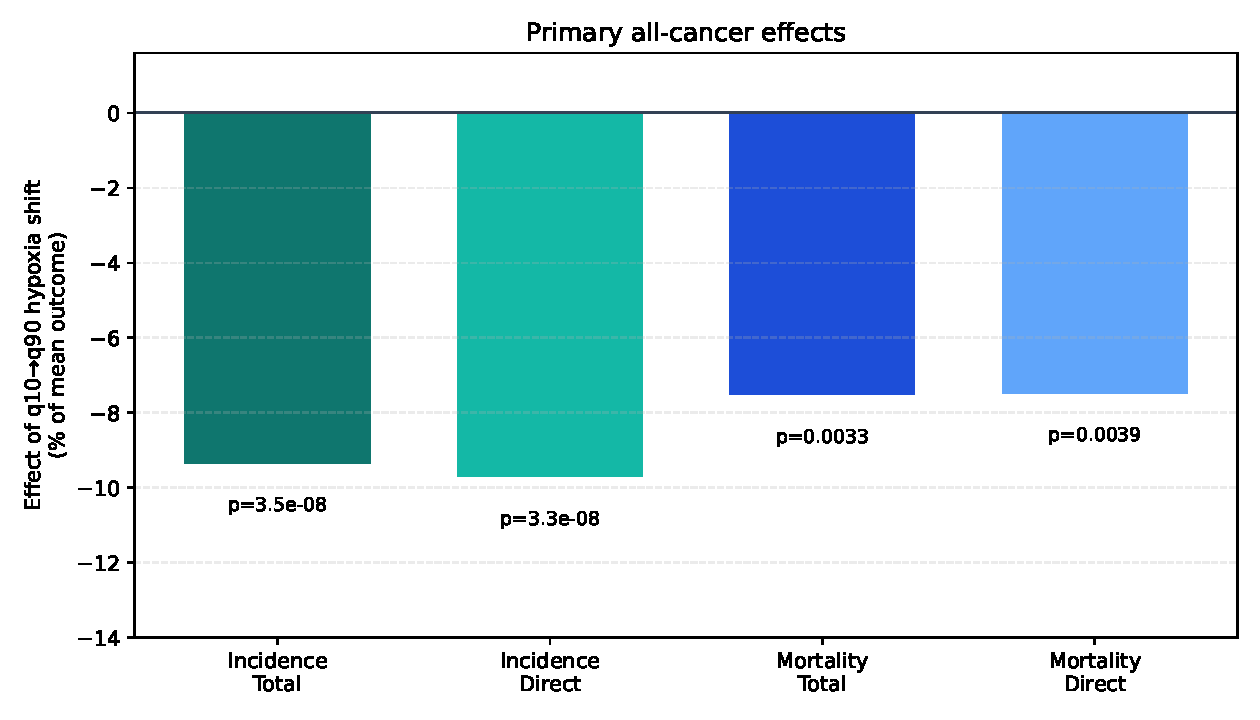
\includegraphics[width=0.78\textwidth]{../outputs/report/paper_assets/primary_effects.pdf}
  \caption{All-cancer effect sizes expressed as the change in outcome induced by shifting hypoxia burden from the 10th to the 90th percentile, normalized by the mean outcome.}
\end{figure}

The repository also exports dose-response curves under the fitted partial-linear models. These curves are linear by construction in the treatment coordinate but remain useful as intervention-style visual summaries because the nuisance adjustment is high dimensional and learned from the transferred feature space.

\begin{figure}[H]
  \centering
  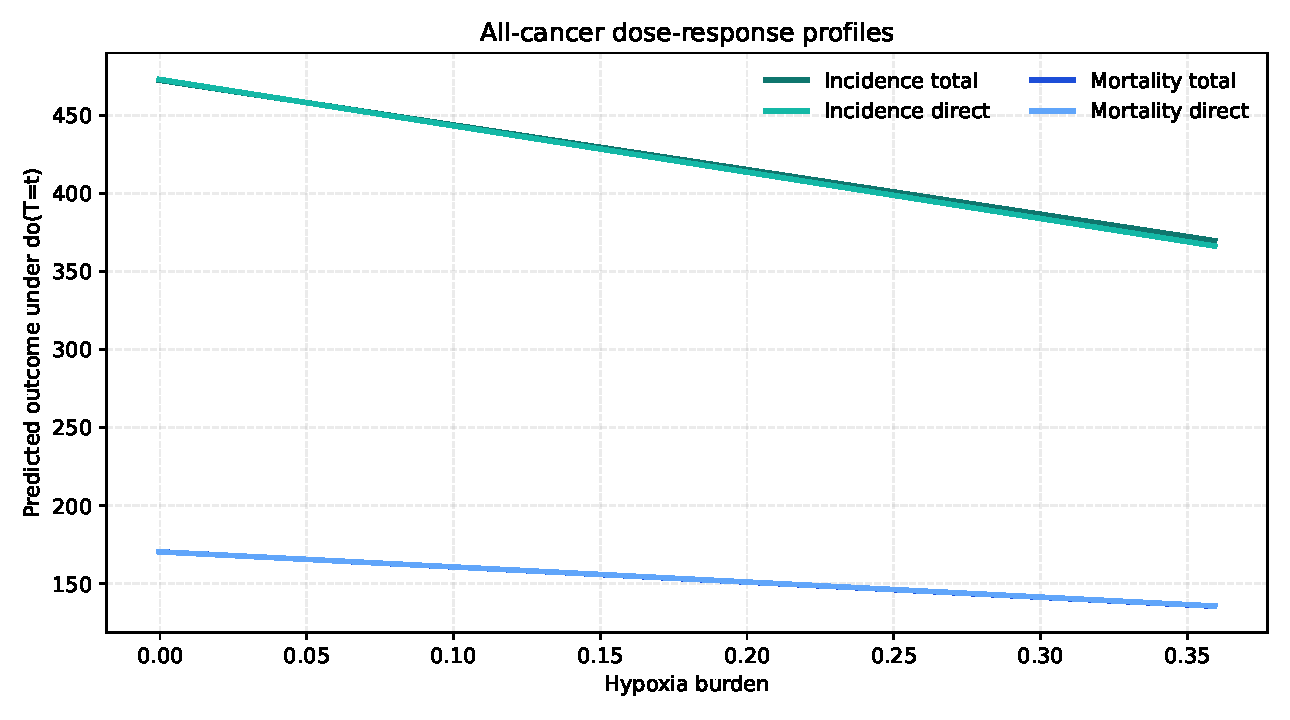
\includegraphics[width=0.82\textwidth]{../outputs/report/paper_assets/dose_response_all_cancer.pdf}
  \caption{Estimated intervention curves for the primary all-cancer models.}
\end{figure}

\section{Site-level heterogeneity}
A key reason to keep the representation layer separate from the causal head is endpoint transfer. Once a county embedding is pretrained, the same representation can be re-used across multiple disease endpoints. That is exactly what happens here: the model is fit not only for all-cancer outcomes but also for site-specific incidence and mortality endpoints with sufficient support.

The incidence results are especially informative. Lung and bronchus incidence shows the strongest negative signal, followed by colon and rectum, breast, urinary bladder, and kidney/renal pelvis. Mortality is more heterogeneous: lung and bronchus remains strongly negative, while prostate mortality shows a positive association in this ecological setting, underscoring that endpoint-specific interpretation matters.

\begin{table}[H]
\centering
\caption{Site-level incidence total-effect estimates}
\resizebox{0.92\textwidth}{!}{%
\begin{tabular}{lrrrr}
\toprule
Site & $N$ & q10$\rightarrow$q90 effect & 95\% CI & $p$ \\
\midrule
Prostate & 981 & -2.7 & [-8.8, 3.5] & 0.3937 \\
Lung and Bronchus & 976 & -15.2 & [-20.0, -10.4] & 7.4e-10 \\
Male and Female Breast & 975 & -7.8 & [-12.3, -3.2] & 0.0008 \\
Colon and Rectum & 954 & -12.4 & [-18.8, -6.0] & 0.0001 \\
Melanomas of the Skin & 801 & -0.4 & [-8.6, 7.8] & 0.9217 \\
Urinary Bladder & 797 & -7.2 & [-12.9, -1.5] & 0.0136 \\
Kidney and Renal Pelvis & 786 & -5.1 & [-9.5, -0.7] & 0.0217 \\
Non-Hodgkin Lymphoma & 754 & -2.2 & [-8.8, 4.4] & 0.5144 \\
\bottomrule
\end{tabular}%
}
\end{table}

\begin{table}[H]
\centering
\caption{Site-level mortality total-effect estimates}
\resizebox{0.92\textwidth}{!}{%
\begin{tabular}{lrrrr}
\toprule
Site & $N$ & q10$\rightarrow$q90 effect & 95\% CI & $p$ \\
\midrule
Lung and Bronchus & 1,103 & -11.1 & [-14.9, -7.2] & 1.5e-08 \\
Colon and Rectum & 866 & -2.5 & [-10.5, 5.5] & 0.5431 \\
Pancreas & 703 & 0.6 & [-3.8, 5.0] & 0.7800 \\
Male and Female Breast & 653 & 3.2 & [-1.2, 7.7] & 0.1550 \\
Prostate & 562 & 13.4 & [6.3, 20.5] & 0.0002 \\
Liver and Intrahepatic Bile Duct & 499 & -4.3 & [-9.0, 0.5] & 0.0805 \\
Leukemias & 475 & 1.2 & [-5.5, 7.8] & 0.7328 \\
Non-Hodgkin Lymphoma & 415 & -0.0 & [-5.4, 5.3] & 0.9891 \\
\bottomrule
\end{tabular}%
}
\end{table}

\begin{figure}[H]
  \centering
  \begin{subfigure}[t]{0.49\textwidth}
    \centering
    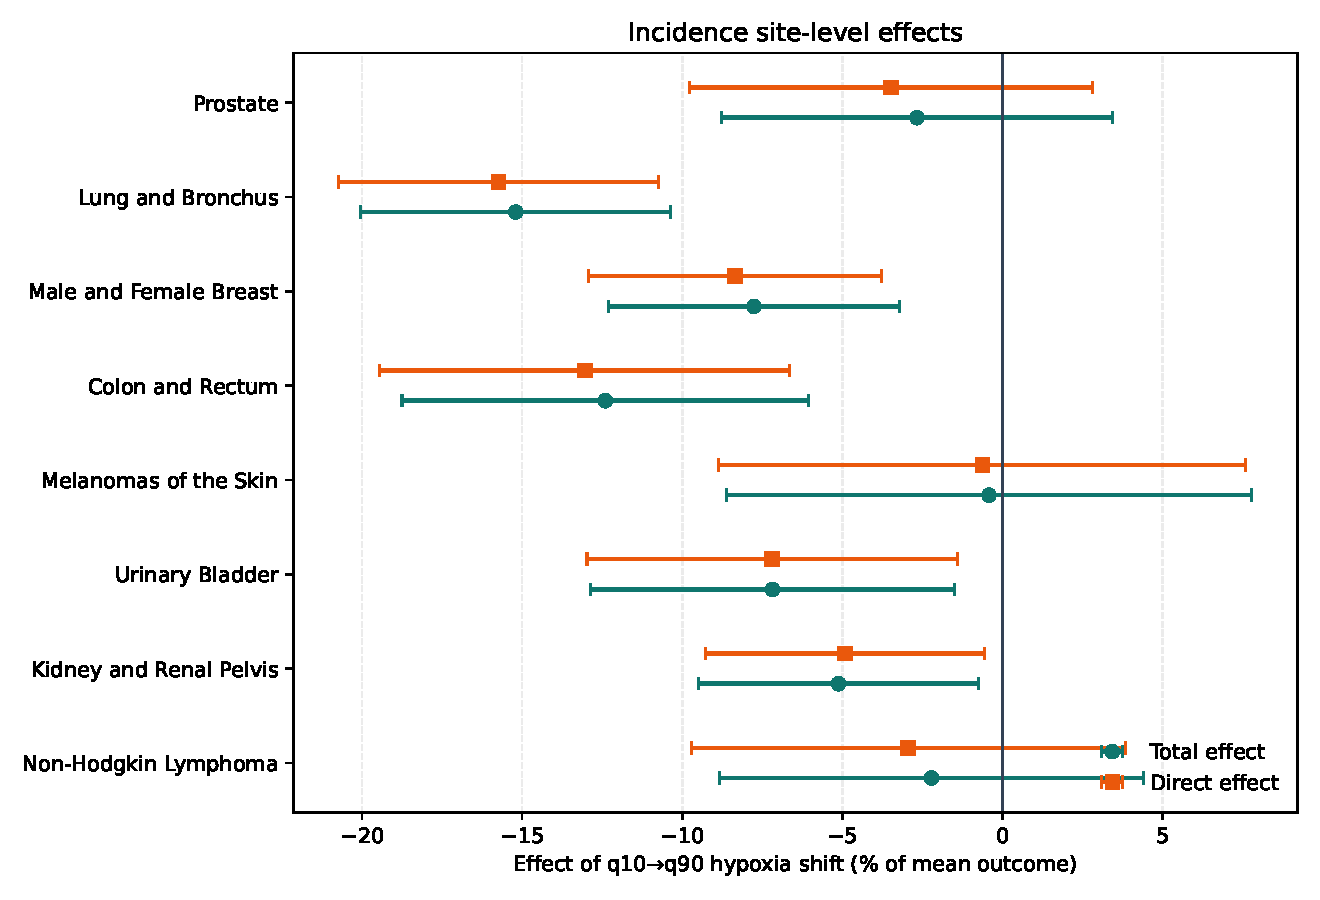
\includegraphics[width=\textwidth]{../outputs/report/paper_assets/site_effects_incidence.pdf}
    \caption{Incidence endpoints}
  \end{subfigure}
  \hfill
  \begin{subfigure}[t]{0.49\textwidth}
    \centering
    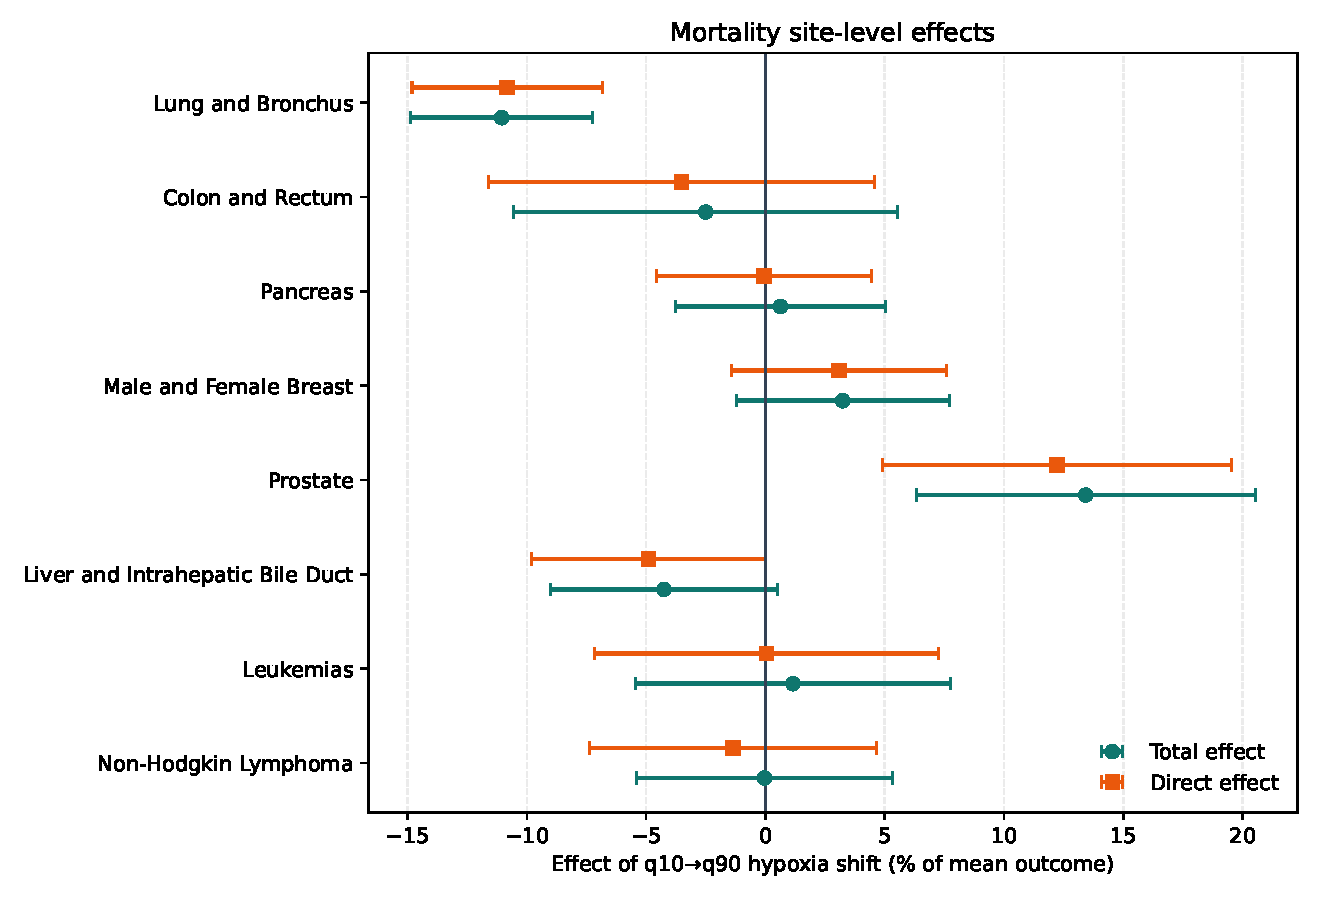
\includegraphics[width=\textwidth]{../outputs/report/paper_assets/site_effects_mortality.pdf}
    \caption{Mortality endpoints}
  \end{subfigure}
  \caption{Site-level effect heterogeneity. Points and intervals are expressed on the normalized q10$\rightarrow$q90 treatment-shift scale.}
\end{figure}

\section{Robustness and failure modes}
The current saved robustness suite is targeted rather than exhaustive: the repository contains \PhaseFourSeedsTested{} seed in the saved seed-sensitivity output and \PhaseFourStatesTested{} state in the saved leave-one-state-out summary. This is sufficient to demonstrate the robustness API and reporting flow, but it is not yet a publication-grade sensitivity battery.

Even so, the relevant technical point is that robustness is integrated into the causal stack rather than appended as a rhetorical afterthought. The same pipeline can be extended to spatial blocks, placebo exposures, negative-control outcomes, and richer leave-region-out analyses once additional environmental and healthcare-access covariates are added.

A separate failure mode is overfitting in the representation learner. In this project, that risk is partially accepted. The present objective is to demonstrate a real causal-AI scaffold and to motivate richer data collection. In other words, mild overfit in the representation layer is tolerable so long as the final causal head remains transparent and the next study design is materially improved.

\section{Why this is already fundable}
The prototype is fundable because it solves the right technical problems in the right order. It defines a biologically motivated exposure, trains a modern tabular encoder rather than relying on hand-crafted summary statistics alone, connects that encoder to an orthogonal causal estimator, and reveals where endpoint heterogeneity is likely to matter. That is already enough to support a stronger second-stage study.

The natural scale-up is a person-level longitudinal design with direct oxygen and physiology measurements. With wearable or digital-health partners, one can replace the current county proxy with a treatment trajectory such as
\begin{align}
T_{it} = f(\mathrm{SpO}_2, \text{altitude}, \text{sleep}, \text{activity}, \text{cardiorespiratory state})_{it},
\end{align}
and estimate effects on incident disease, progression, or survival outcomes under time-varying exposure. The representation model can also scale naturally: person-time windows can be tokenized analogously to county features, pretraining can absorb larger multimodal streams, and the causal head can move toward longitudinal orthogonal estimation.

From a fundraising perspective, the county analysis therefore de-risks four specific things: treatment definition, endpoint prioritization, model architecture, and reporting discipline. It is not the final study, but it is exactly the kind of prototype that makes a larger study technically credible.

\section{Conclusion}
The key message of this paper is simple. OxyFormer is no longer just a demonstration of ridge-based DML on a county table. It is now a bona fide causal-AI system with attention-based transformer pretraining, transferred tabular embeddings, orthogonal continuous-treatment estimation, and site-level endpoint reuse. That architecture is already informative on its own, and it points directly toward the next fundable experiment: direct oxygen and health measurement at person scale.


\end{document}
